\documentclass{standalone}
\usepackage{tikz}
\usepackage{ctex,siunitx}
\setCJKmainfont{Noto Serif CJK SC}
\usepackage{tkz-euclide}
\usepackage{amsmath}
\usetikzlibrary{patterns, calc,3d}
\usetikzlibrary {decorations.pathmorphing,decorations.pathreplacing,decorations.shapes}
\begin{document}
\small
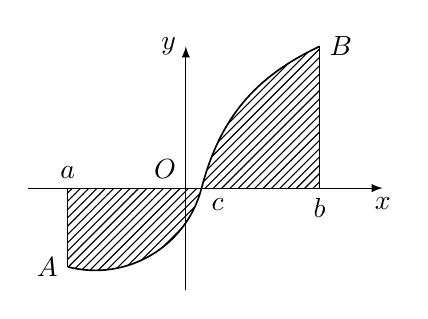
\begin{tikzpicture}[>=latex,scale=1.0]
  \draw[->](-2,0)--(2.5,0)node[below]{$x$};
  \draw[->](0,-1.3)--(0,1.8)node[left]{$y$};
  \draw[semithick](-1.5,-1)node[left]{$A$}to[bend right=45](0.2,0)node[below right]{$c$}to[bend left=25](1.7,1.8)node[right]{$B$};
  \draw(-1.5,-1)--(-1.5,0)node[above]{$a$};
  \draw(1.7,1.8)--(1.7,0)node[below]{$b$};
  \fill[pattern=north east lines](-1.5,0)--(-1.5,-1)to[bend right=45](0.2,0)to[bend left=25](1.7,1.8)--(1.7,0);
  \node at (0,0)[above left]{$O$};
\end{tikzpicture}
\end{document}